\documentclass[12pt, reqno]{amsart}
\paperheight=11in
\paperwidth=8.5in
\usepackage[margin = 1 in]{geometry}
\usepackage{float}
\usepackage{fancyhdr}
\usepackage{physics}
\usepackage{graphicx}
\usepackage{hyperref}
\usepackage{fancyvrb}
\usepackage{mathtools}
\usepackage{wrapfig}
\raggedbottom

\begin{document}

\title{CFDG \quad Vorticity-Streamfunction Solver \quad Jacob Ivanov}
\maketitle
\section{Introduction}
Oftentimes, the onboarding of a new researcher within computational fluids, or computational groups in general, is hampered by a lack of understanding on how to actually implement a method that is usually described in a page or two within a textbook. As a case in point, a basic description of the Voriticity-Streamfunction method is described in Section 7.2.4 of Ferziger's \textit{Computational Methods for Fluid Dynamics}, and can be read in 10 minutes. However, implementing a Spectral variation of that method (as well as quite a few additions) has been the main focus of my research with Dr.\ Georgios Matheou within the Computational Fluid Dynamics Group (CFDG) over the course of the last year.

The goal of this documentation is to create an understandable guide to implementing this Spectral Vorticity-Streamfunction method, which another new researcher can follow and expand upon for themselves, and in the process gain familiarity with the basic requirements of computational implementations in general.

\section{Spectral Vorticity-Streamfunction Method}
\subsection{Governing Equations}
Starting from the very beginning, Issac Newton determined that $\vec{F} = m \vec{a}$, from which the 2D Navier-Stokes equations can be trivially derived\footnote{Left as an exercise to the reader. In all seriousness, this is very well explained in any introductory Fluid Mechanics textbook.}:
\begin{equation}
    \pdv{u_x}{t} + u_x \pdv{u_x}{x} + u_y \pdv{u_x}{y} = - \frac{1}{\rho} \pdv{p}{x} + \nu \left( \pdv[2]{u_x}{x} + \pdv[2]{u_x}{y} \right)
\end{equation}
\begin{equation}
    \pdv{u_y}{t} + u_x \pdv{u_y}{x} + u_y \pdv{u_y}{y} = - \frac{1}{\rho} \pdv{p}{y} + \nu \left( \pdv[2]{u_y}{x} + \pdv[2]{u_y}{y} \right)
\end{equation}
where the fluid velocity components are $\vec{u} = \langle u_x, u_y \rangle$, $p$ is the fluid pressure, $\nu$ is the kinematic viscosity, and $\rho$ is the fluid density. By differentiating (1) with respect to $y$, (2) with respect to $x$, and obtaining the difference, we can eliminate the pressure term, and obtain the following\footnote{Making the assumption of incompressiblity, i.e. $\rho = c$, $\nabla \cdot \vec{u} = 0$. Additionally, this derivation also works with some conservative body force $\vec{g}$ acting on the fluid, which has been ignored.}:
\begin{equation}
    \begin{aligned}
    \pdv{}{t} \left[ \pdv{u_x}{y} - \pdv{u_y}{x} \right] &+ (u_x + 1) \frac{\partial^2 u_x}{\partial x \partial y} - (u_y + 1) \frac{\partial^2 u_y}{\partial x \partial y} \\
    & + \pdv{u_y}{y} \pdv{u_x}{y} - \pdv{u_x}{x} \pdv{u_y}{x} + \nu \left( \pdv{}{x} \left[ \nabla^2 u_y \right] - \pdv{}{y} \left[ \nabla^2 u_x \right] \right) = 0
    \end{aligned}
\end{equation}
From there, we can use the streamfunction $\psi$ and vorticity $\omega$ as intermediate variables, which are defined below:
\begin{equation}
    u_x = + \pdv{\psi}{y}, \quad u_y = - \pdv{\psi}{x}
\end{equation}
\begin{equation}
    \omega = \nabla \times \vec{u} = \pdv{u_y}{x} - \pdv{u_x}{y} = - \nabla^2 \psi
\end{equation}
As a result, we can obtain the respective Streamfunction and Vorticity Transport formulations of the 2D Navier-Stokes equations.
\begin{equation}
    \pdv{}{t} \left[ \nabla^2 \psi \right] + \pdv{\psi}{y} \pdv{}{x} \left[ \nabla^2 \psi \right] - \pdv{\psi}{x} \pdv{}{y} \left[ \nabla^2 \psi \right] = \nu \nabla^2 \left[ \nabla^2 \psi \right]
\end{equation}
\begin{equation}
    \pdv{\omega}{t} + u_x \pdv{\omega}{x} + u_y \pdv{\omega}{y} = \nu \nabla^2 \omega
\end{equation}
Due to it's compactness, we will use Eq. (7) going forward. Additionally, though this method is referred to as the Vorticity-Streamfunction method, it is not necessary to calculate the Streamfunction intermediately.

\subsection{Spectral Vorticity Transport Equation}
Within this solver, we will be using spectral methods to time-step and obtain derivatives, and as a result, we need to rewrite Eqs. (5) and (7).
\begin{equation}
    \pdv{\Omega}{t} + \nu (k_p^2 + k_q^2) \Omega = - \mathcal{F}_{+2} \left[ u_x \pdv{\omega}{x} + u_y \pdv{\omega}{y} \right]
\end{equation}
\begin{equation}
    u_x = \mathcal{F}_{-2} \left[ U_x \right] = \mathcal{F}_{-2} \left[ + \frac{\underline{i} k_q \Omega}{k_p^2 + k_q^2} \right], \quad u_y = \mathcal{F}_{-2} \left[ U_y \right] = \mathcal{F}_{-2} \left[ - \frac{\underline{i} k_p \Omega}{k_p^2 + k_q^2} \right]
\end{equation}
\begin{equation}
    \pdv{\omega}{x} = \mathcal{F}_{-2} \left[\underline{i} k_p \Omega \right], \quad \pdv{\omega}{y} = \mathcal{F}_{-2} \left[\underline{i} k_q \Omega \right]
\end{equation}
where $\underline{i}$ is the imaginary unit, $k_p$ and $k_q$ are the spectral $x$- and $y$-derivative operators, $\Omega$, $U_x$, and $U_y$ are the frequency version of $\omega$, $u_x$, and $u_y$, respectively, and $\mathcal{F}_{+2}$, $\mathcal{F}_{-2}$ are the forward and backward 2D Fourier Transforms, respectively. Unfortunately, we need to repeatedly use the Fourier Transform between physical/frequency space to compute the non-linear product in the convection term.

Time-stepping Eqs. (8)-(10) is possible, but due to the combination of first- and second-order derivatives, numerical stability is difficult to maintain. As a result, we can further modify the Spectral Vorticity Transport Equation to use an integrating factor:
\begin{equation}
    \Xi(t_n) = \exp \left[ \nu (k_p^2 + k_q^2) t_n \right]
\end{equation}
\begin{equation}
    \pdv{}{t_n} \left[ \Xi(t_n) \cdot \Omega \right] = - \underline{i} \Xi(t_n) \cdot \mathcal{F}_{+2} \left[ u_x \pdv{\omega}{x} + u_y \pdv{\omega}{y} \right]
\end{equation}
Unfortunately, because $\partial \Xi/\partial t$ is strictly positive, as $t_n$ increases, the $\Xi(t_n)$ variable will become gradually less precise, and eventually will overflow due to the floating point format it is stored as computationally. As a result, we can make our final modification\footnote{This change is legitimate because it is equivalent to `reseting' our $\Xi(t_n) \Omega$ variable by pre-multiplying by $\Xi(-t_n)$ at the beginning of each integration timestep.} to our Spectral Vorticity Transport equation:
\begin{equation}
    \pdv{}{t_n} \left[ \Xi(c_s \Delta t) \cdot \Omega \right] = - \underline{i} \Xi(c_s \Delta t) \cdot \mathcal{F}_{+2} \left[ u_x \pdv{\omega}{x} + u_y \pdv{\omega}{y} \right]
\end{equation}
where $c_s$ is the time supstep fraction for the Runge-Kutta integration method described later, and $\Delta t$ is the time-step.

\subsection{Initial Condition}
While any smooth $2 \pi$-periodic initial velocity field would work, Taylor-Green flow is a natural choice, and gives us the ability to test against the analytical solution over time. Taylor-Green flow is described by:
\begin{equation}
    \begin{cases}
        u_x(t, x, y) = + e^{-2 \nu t} \cos(\beta x) \sin(\beta y) \\
        u_y(t, x, y) = - e^{-2 \nu t} \sin(\beta x) \cos(\beta x)
    \end{cases}
\end{equation}
where $\beta$ is a scaling integer constant. The vortex wavelength will be $2 \pi / \beta$. However, any perturbation to the initial condition will cause the flow to destabilize, resulting in turbulence. As a result, we will set the initial condition instead to the following:
\begin{equation}
    \begin{cases}
        u_x(t = 0, x_i, y_j) = + \cos(\beta x_i) \sin(\beta y_j) + \gamma_x \\
        u_y(t = 0, x_i, y_j) = - \sin(\beta x_i) \cos(\beta y_j) + \gamma_y
    \end{cases}
\end{equation}
where $\gamma_x$ and $\gamma_y$ represent uniform \texttt{rng}-generated perturbations to the $x$- and $y$-velocity. Its magnitude must be relatively small, and has been set to 0.02 for this project.

\subsection{Runge-Kutta Integration Method}
Now that we have the final form of our governing equations, as well as an initial condition, we need a way to integrate them over time. One might immediately think of something like Euler's Method, where you can timestep as follows:
\begin{equation}
    y_{n + 1} = y_n + \Delta t \cdot f(t_n, y_n)
\end{equation}
where $f = \dd y/ \dd t$. Euler's Method is actually a first-order version of a Runge-Kutta (RK) method, but is unstable for typical fluid dynamics problems\footnote{Consult Chapter 7: ``Stability of Linear Systems'' within Lomax's \textit{Fundamentals of Computational Fluid Dynamics} for a full explanation.}, and as a result, we will need to use a higher order RK method. In general\footnote{There are more advanced variations of RK Methods, ranging from implicit, adaptive, etc. that are descibed well in the Wikipedia Article on \href{https://en.wikipedia.org/wiki/Runge\%E2\%80\%93Kutta_methods}{RK Methods}. Within this project, we have only done explicit forms.}, RK methods are described by three coefficient matrices: $\mathbf{a}$, $\mathbf{b}$, and $\mathbf{c}$, which are referred to as the RK Matrix, Weights Matrix, and Nodes Matrix. The solution for the next time-step can be constructed as follows: 
\begin{equation}
    \begin{dcases}
        y_{n+1} = y_n + \Delta t \sum_{i = 1}^s \left[ b_i k_i \right] \\
        k_i = f \left(t_n + c_i \Delta t, y_n + \Delta t \sum_{j = 1}^{i - 1} \left[ a_{ij} k_j \right] \right)
    \end{dcases}
\end{equation}
We will specifically use  Wray's Method\footnote{Also referred to as Van der Houwen's Method. The autonomous version of which was described within \textit{Spectral Methods for the Navier-Stoes Equations with One Infinite and Two Periodic Directions} by Spalart et al.}, with a Butcher Table as follows:

\begin{equation}
    \begin{array}{c | c}
        \mathbf{c} & \mathbf{a} \\
        \hline
        & \mathbf{b}
    \end{array} = \begin{array}{c | cccc }
        0 & 0 & 0 & 0 \\
        8/15 & 8/15 & 0 & 0\\
        2/3 & 1/4 & 5/12 & 0\\
        \hline
            & 1/4 & 0 & 3/4
    \end{array}
\end{equation}
However, we cannot pick any arbitrary $\Delta t$ and maintain stability, and so we use the Courant-Friedrich-Lewy (CFL) condition. Prior to starting an RK3 step, we find the $\max \left[ u_x \right]$ and $\max \left[ u_y \right]$, and find $\Delta t$ as follows:
\begin{equation}
    \Delta t = \frac{\Delta x \Delta y}{\Delta y \max \left[ u_x \right] + \Delta x \max \left[ u_y \right]}
\end{equation}

\subsection{Particle Transport}
Consider a point particle dropped into a flow. If the particle is non-inertial, it will instantaneouly be travelling at the same velocity and direction as the flow surrounding it.
\begin{equation}
    \vec{v}(t, \vec{x}_p) = \vec{u}(t, \vec{x}_p)
\end{equation}
where $\vec{x}$ is the particle position vector, $\vec{u}$ is fluid velocity vector, and $\vec{v}$ is the particle velocity vector. As a result, the particle position can be directly time-stepped by updating the particle position by its velocity. 
However, if the particle is inertial, the particle velocity and fluid velocity will no longer be instantaneously equal, but rather, will be described by the following:
\begin{equation}
    \dv{\vec{v}}{t} = \frac{1}{\tau} (\vec{u} - \vec{v}) + 3 
    \vec{a}
\end{equation}
where $\vec{a}$ is the fluid acceleration\footnote{It should be noted that particle transport is by default Lagrangian rather than Eulerian, and as a result, the acceleration experienced by a fluid element at position $\vec{x}$ is $\vec{a} = \mathrm{D} \vec{u}/\mathrm{D} t \neq \dd \vec{u}/ \dd t$, or more explicitly:
\[ \vec{a}(\vec{x}) = \frac{\mathrm{D} \vec{u}}{\mathrm{D} t} = \dv{\vec{u}}{t} + (\nabla \cdot \vec{u}(\vec{x}))\vec{u}(\vec{x}) \] If this is unintuitive to you, consider a steady, but non-uniform fluid velocity field $\vec{u}(\vec{x})$. Since it is steady, $\dd \vec{u} / \dd t = 0$, but is the fluid acceleration zero everywhere?}, and $\tau$ is the non-dimensional inertial time\footnote{The inertial time $\tau$ is dependent on the particle geometry, fluid viscosity, particle/fluid density ratio, etc.\ but here will be assumed to be just an independent constant.}. Due to the coupled nature of Eq. (20), the following Predictor-Corrector (PC) scheme\footnote{This scheme is from \textit{Effect of Bubble Size on Lagrangian Pressure
Statistics in Homogeneous Isotropic Turbulence} by M.H. Bappy et al., but excludes bubble buoyancy.} was implemented:

Predictor:
\begin{align}
    \vec{x}_{n + \alpha} &= \vec{x}_n + \Delta t \cdot \vec{v}_n\\
    \vec{u}_{n + \alpha} &= \vec{u}(t_n, \vec{x}_{n + \alpha})\\
    \vec{v}_{n + \alpha} &= \dfrac{\vec{v}_n + \Delta t \left[ \dfrac{\vec{u}_{n + \alpha}}{\tau} + 3\vec{a}_n \right]}{1 + \dfrac{\Delta t}{\tau}}
\end{align}

Corrector:
\begin{align}
    \vec{x}_{n + 1} &= \vec{x} + \frac{\Delta t}{2} \left( \vec{v}_n + \vec{v}_{n + \alpha} \right) \\
    \vec{u}_{n+1} &= \vec{u} ( t_{n+1}, \vec{x}_{n+1})\\
    \vec{a}_{n+1} &= \vec{a} (t_{n+1}, \vec{x}_{n+1})\\
    \vec{v}_{n+1} &= \dfrac{1}{1 + \frac{\Delta t}{2 \tau}} \left[ \vec{v}_n + \frac{\Delta t}{2} \left( 3 (\vec{a}_n + \vec{a}_{n+1} ) + \frac{\vec{u}_n + \vec{u}_{n+1} - \vec{v}_n}{\tau} \right) \right]
\end{align}
It can be seen that in the non-inertial case, where $\tau = 0$, this PC scheme degenerates to Heun's Method.

\subsection{Spectral Interpolation}
Ironically, though described last in the this project documentation's methods, this was the first aspect of the project that was completed. In order to obtain accurate interpolated values for fluid velocity, acceleration, etc.\ at locations in between the grid points, we can exploit the periodic nature of the flow and use Spectral Interpolation, where we rebuild the point's value by using the Fourier Coefficients.

Assuming the values of a discrete periodic function $y_i(x_i)$ on domain $x_i \in [0, 2 \pi)$, the Fourier Transform of $y_i$ is $Y_p = \mathcal{F}_{+1} \left[ y_i \right]$. An interpolating polynomial can be constructed as:
\begin{equation}
    p(x) = \frac{1}{N} \sum_p \left[ Y_p e^{\underline{i} k_p x} \right]
\end{equation}
$p(x)$ can be evaluated at the target location in order to find the interpolated value at the location. In higher dimensions, this will need to repeated across all $x$, then across a single $y$, etc.

\section{Results}
In total, we have a Spectral Voriticity-Streamfunction method Navier-Stokes solver with inertial particle transport. The script \texttt{vorticity\_streamfunction\_solver.py} can run to obtain similar results:

\begin{figure}[H]
    \centering
    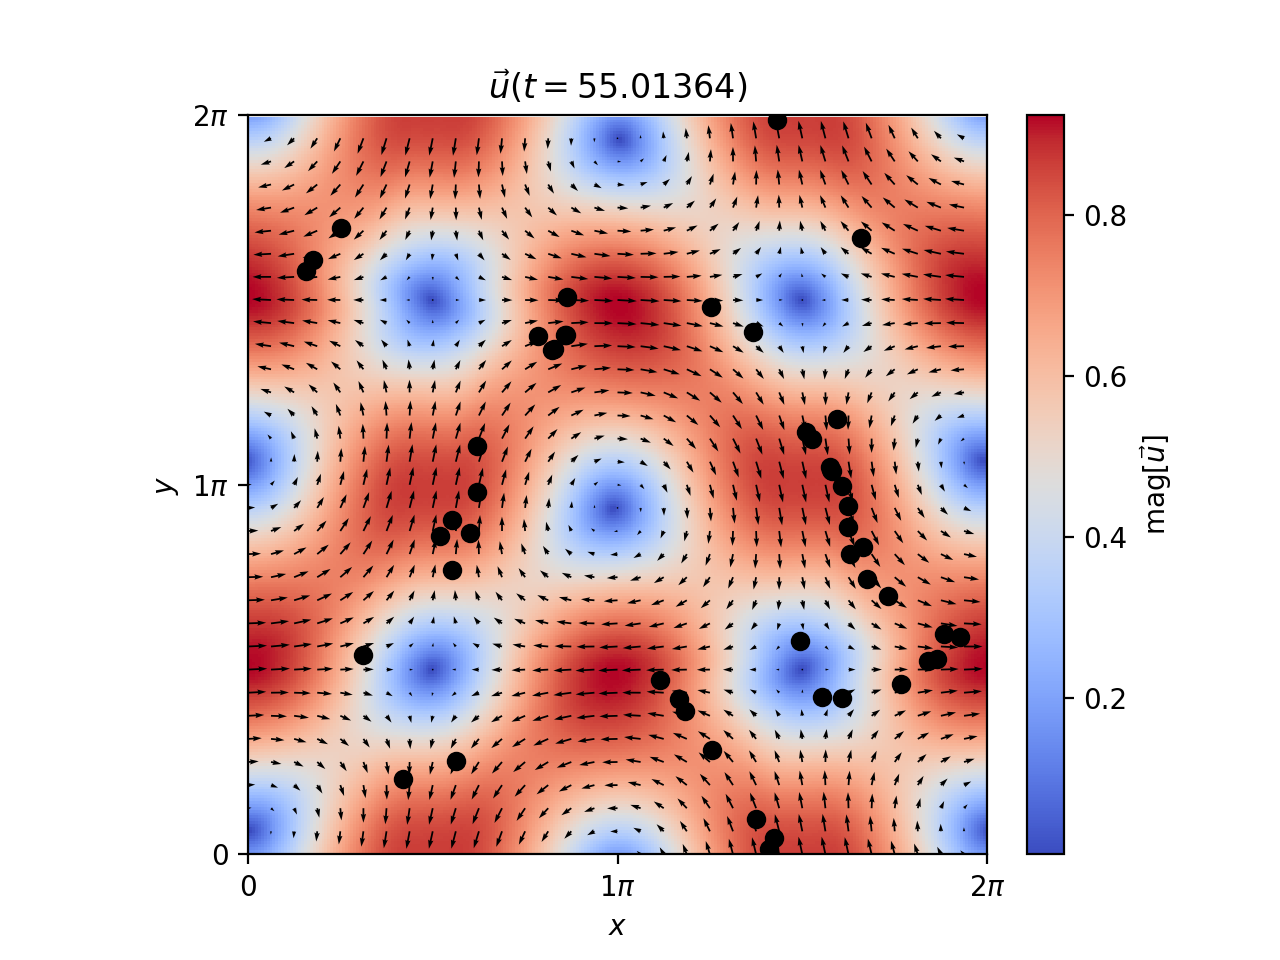
\includegraphics[width = 1\linewidth]{Vorticity-Steamfunction.png}
\end{figure}

By tracking each particle for the time period following destabilization, once turbulence is initiated, it can be seen that these particles follow independent and chaotic paths.

\begin{figure}[H]
    \centering
    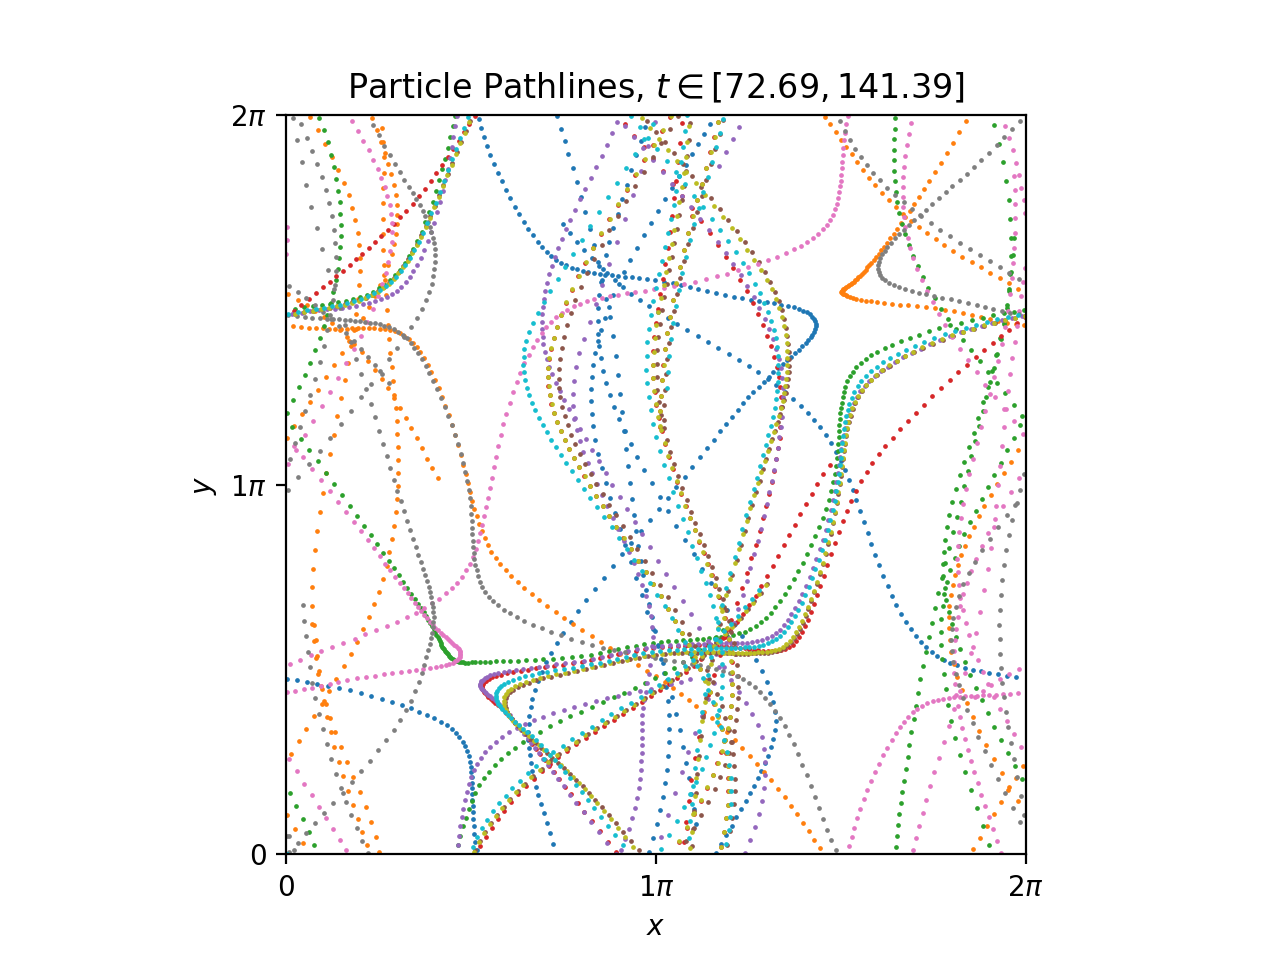
\includegraphics[width = 1\linewidth]{Particle Pathlines.png}
\end{figure}



\section{Verification Tests}
\subsection{Verification of Spectral Differentiation} 
The first thing we need to verifiy is our ability to spectrally differentiate and anti-differentiate. 

The Fourier Transform is defined as the following:
\begin{equation}
    u_i = \sum_i \left[ U_p \cdot e^{\underline{i} k_p x_i} \right]
\end{equation}
The derivative can be found as follows:
\begin{equation}
    \dv{u_i}{x} = \sum_i \left[ \underline{i} k_p U_p \cdot e^{\underline{i} k_p x_i} \right] = \underline{i} k_p \sum_i \left[ U_p \cdot e^{\underline{i} k_p x_i} \right]
\end{equation}
As a result, we can see that the spectral derivative operator equivalent for $\dd/\dd x = \underline{i} k_p$. Unfortunately, the exact ordering of the wavenumbers $k_p$ is dependent on the implementation of the Discrete Fourier Transform used. 

Throughout this entire project, development was done with Python, and specfically used the \texttt{numpy.fft} package\footnote{\href{https://pypi.org/project/rocket-fft/}{\texttt{rocket-fft}} was used to make \texttt{numba.njit} aware of \texttt{numpy.fft} functionality. It must be installed, or JIT-compilation disabled within \texttt{vorticity\_streamfunction\_solver.py} or an error will result.}, which uses the following format:
\begin{verbatim}
    k = [0, 1, ...,   M/2-1,     -M/2, ..., -1]   if M is even
    k = [0, 1, ..., (M-1)/2, -(M-1)/2, ..., -1]   if M is odd
\end{verbatim}

where \texttt{M} is the number of grid divisions in the range $x \in [0, 2\pi)$.
An arbitrary periodic formula was chosen, $y = \exp [ \cos(x) ] \sin(x)$, with an analytical derivative $y' = - \exp [ \cos(x) ] \left[ \sin^2(x) - \cos(x) \right]$, and a convergence test was completed by increasing the grid spacing and finding the absolute error between the spectrally differentiated and analytical $y'$.
Figure 1 can be reproduced by executing the script \texttt{spectral\_derivative.py} (runtime: $<1$ s).

\begin{figure}[H]
    \centering
    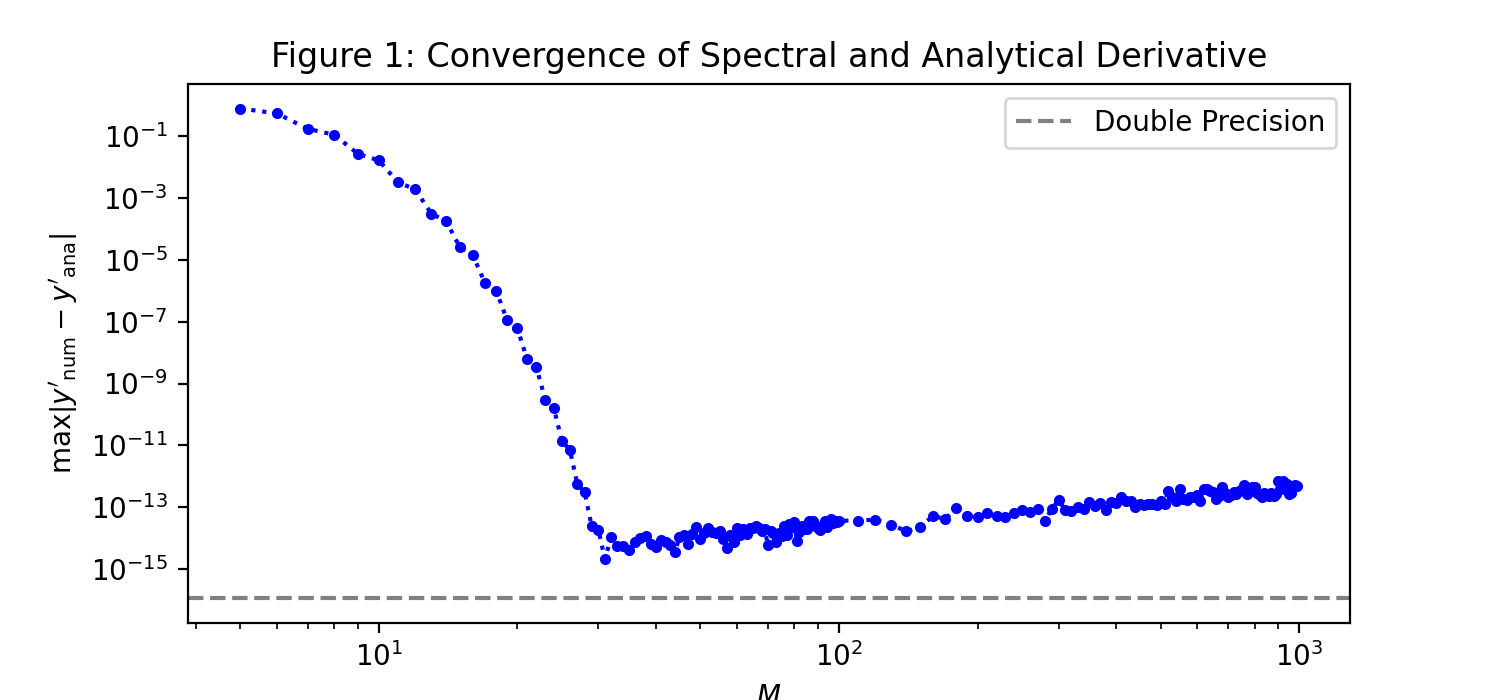
\includegraphics[width = 1\linewidth]{spectral_derivative.png}
\end{figure}

\subsection{Verification of Spectral Poisson Equation}
Now that we have verified our ability to take spectral derivatives, we can tackle the slightly more challenging spectral Poisson Problem. As stated previously, $\omega = - \nabla^2 \psi$. As a result, the frequency versions of voriticity and streamfunctions are related as follows in 2D:
\begin{equation}
    \Omega_{pq} = - \left[ -1 k_p^2 \Psi_{pq} - 1 k_q^2 \Psi_{pq} \right]
\end{equation}
\begin{equation}
    \Psi_{pq} = \frac{\Omega_{pq}}{k_p^2 + k_q^2}
\end{equation}
However, when $p = q = 0$, $\Psi_{00}$ is of form $1/0$. As a result, we are forced to ignore the value of $\Omega_{00}$. As a result, our recovered $\psi_\mathrm{num}$ will have an average of 0, and we will need to correct by the average of the analytical. This is not a problem for our overall solver becasue we never actually need the value of $\psi$, only the derivatives.
\begin{equation}
    \psi_\mathrm{num} - \bar{\psi}_\mathrm{ana} = \mathcal{F}_{-2} \left( \frac{\Omega_{pq}}{k_p^2 + k_q^2} \right)
\end{equation}
Again, we will pick an arbitrary analyitical function for $\psi = \exp[ \cos(x) ] - \sin(y)$ from which we can find a consistent $\omega = e^{\cos(x)} \left[ \cos(x) - \sin^2(x) \right] - \sin(y)$. A convergence test using an $\ell_p$-norm\footnote{In order to quantify the error in a multidimensional matrix, an $\ell_p$-norm is used, defined as: \[ \ell_p [\mathbf{e}] = \left[ \Delta x \Delta y \Delta z \sum_i \sum_j \sum_k \left( e_{ijk}^p \right) \right]^{1/p} \]which is straightforward to simplify for lower dimensions.}, can be completed, yielding results similar to Figure 1, but below the simple error field is plotted for varying computational mesh sizes. Similar to Figure 1, because the lowest mesh shown is finer than $\approx 30$, the error is on the order of machine epsilon already. Figure 2 can be reproduced by executing the script \texttt{spectral\_poisson.py} (runtime $<5$ s).

\begin{figure}[H]
    \centering
    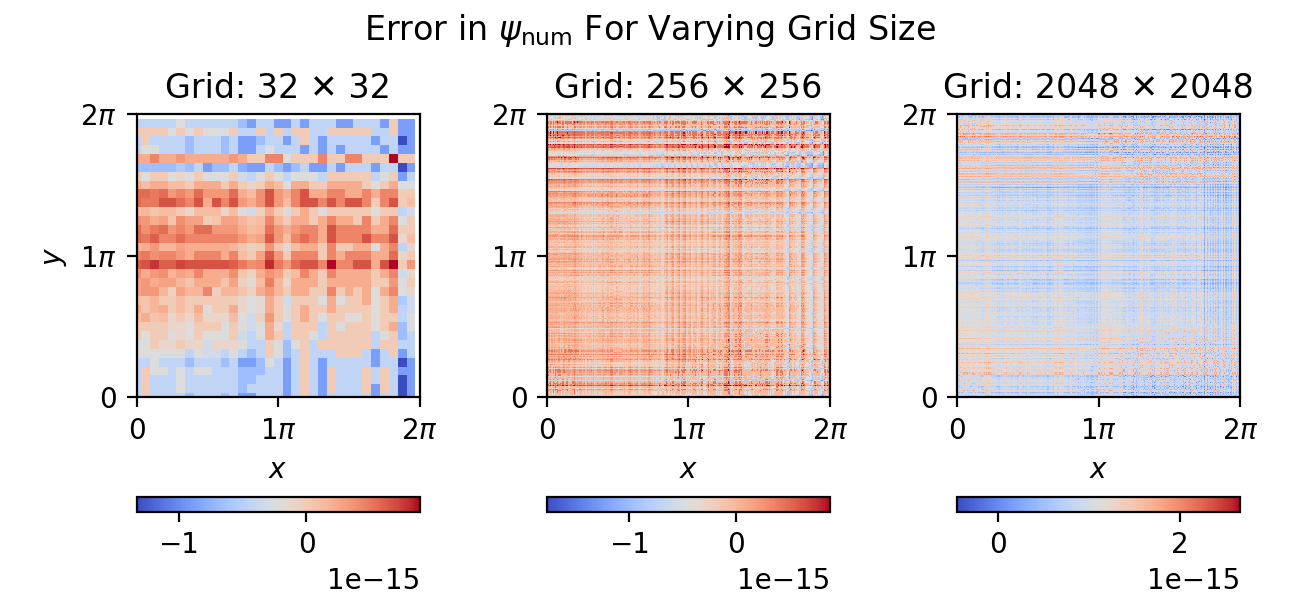
\includegraphics[width = 1\linewidth]{spectral_poisson.png}
\end{figure}

\subsection{Verification of Spectral Interpolation}
In order to verify our Spectral Interpolation method, we will compare the analytical values of the function $f = \exp [ \sin(x) + \sin(y)]$ to our interpolation. This was accomplished in the script \texttt{inter2D\_convergence.py} (runtime $<3$ m).

\begin{figure}[H]
    \centering
    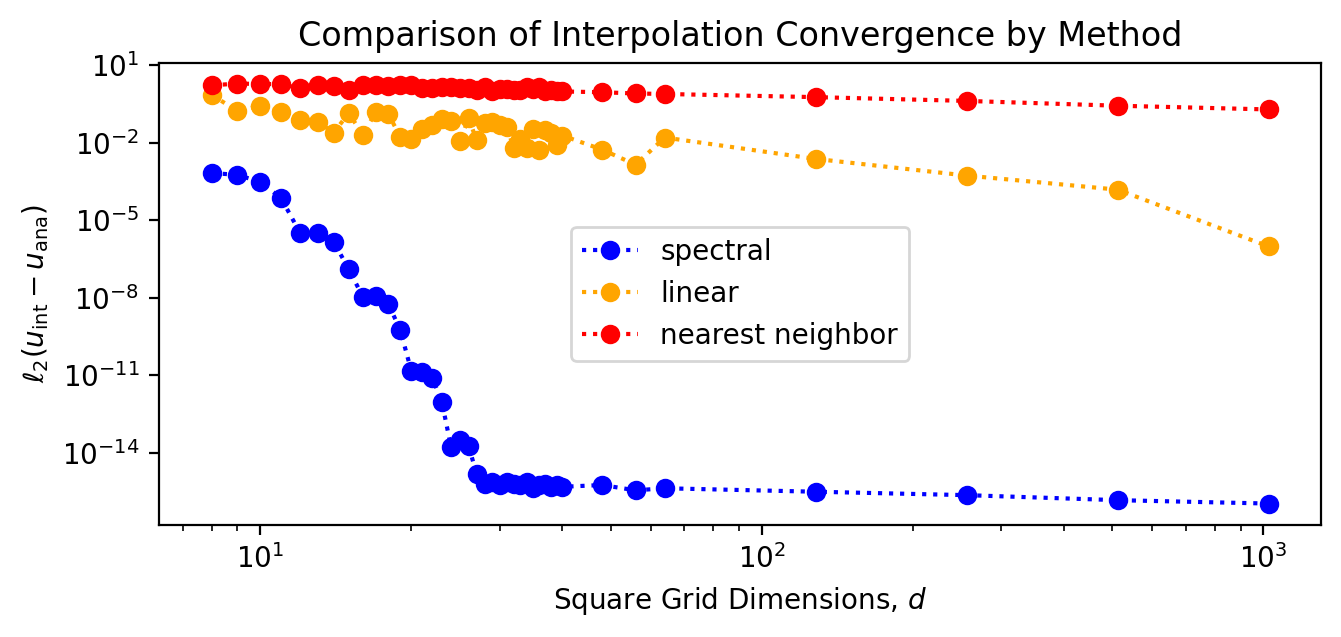
\includegraphics[width = 1\linewidth]{Comparison of Interpolation Convergence by Method.png}
\end{figure}

\subsection{Verification of RK3 Method}
Confident that we have the required ability to compute spectral derivatives and anti-derivatives, and thereby the spectral Poisson equation, we can move on to testing our timestepping mechanism. As was stated previously, we will be using Wray's RK3 method, which after expanding out the Butcher table, cooresponds to
\begin{align}
k_1 &= f(t_n, y_n) \\
k_2 &= f \left(t_n + \frac{8}{15} \Delta t, y_n + \Delta t \cdot \frac{8}{15} k_1 \right) \\
k_3 &= f \left(t_n + \frac{2}{3} \Delta t,  y_n + \Delta t \cdot \left( \frac{1}{4} k_1 + \frac{5}{12} k_2 \right) \right) \\
y_{n + 1} &= y_n + \Delta t \left[ \frac{1}{4} k_1 + \frac{3}{4} k_3 \right]
\end{align}
As before, we find an analytical problem that we can solve, and test against the known solution. The autonomous\footnote{An autonomous ODE's solution is independent of when the initial condition is applied. The RHS has no $t$-dependence.} equation $y' = y$ has the known solution $y(t) = y(0) \cdot e^t$.
\begin{figure}[H]
    \centering
    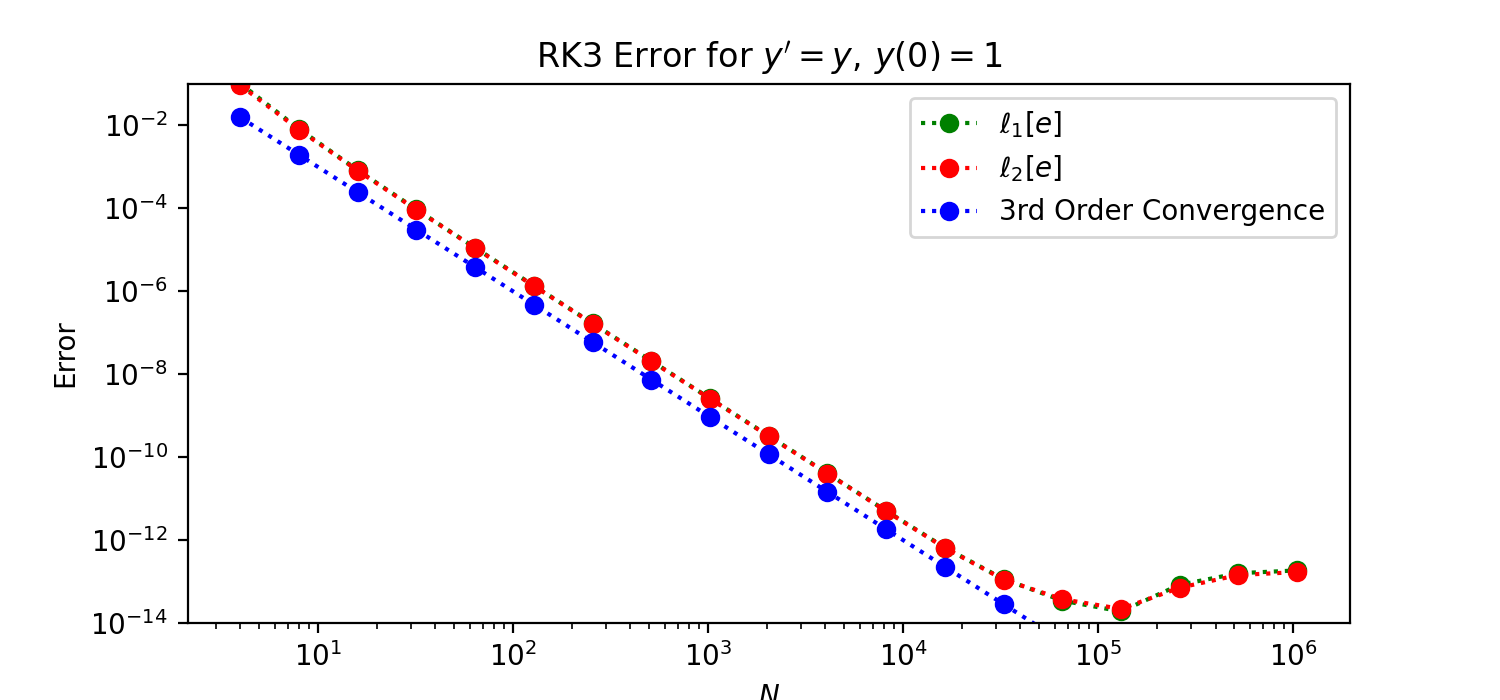
\includegraphics[width = 1\linewidth]{RK3 Error Convergence.png}
\end{figure}
This figure can be reproduced by executing the script \texttt{rk3\_exp.py} (runtime $<1$ s).

Interestingly enough, modifying the form of $f$ can dramatically change the error in the RK integation. The following are equivalent:
\begin{equation}
    \dv{y}{t} = ty \iff \dv{}{t} \left[ \exp \left( - \frac{1}{2} t^2 \right) \cdot y \right] = 0
\end{equation}
But integrating each form shows dramatically different error:

\begin{figure}[H]
    \centering
    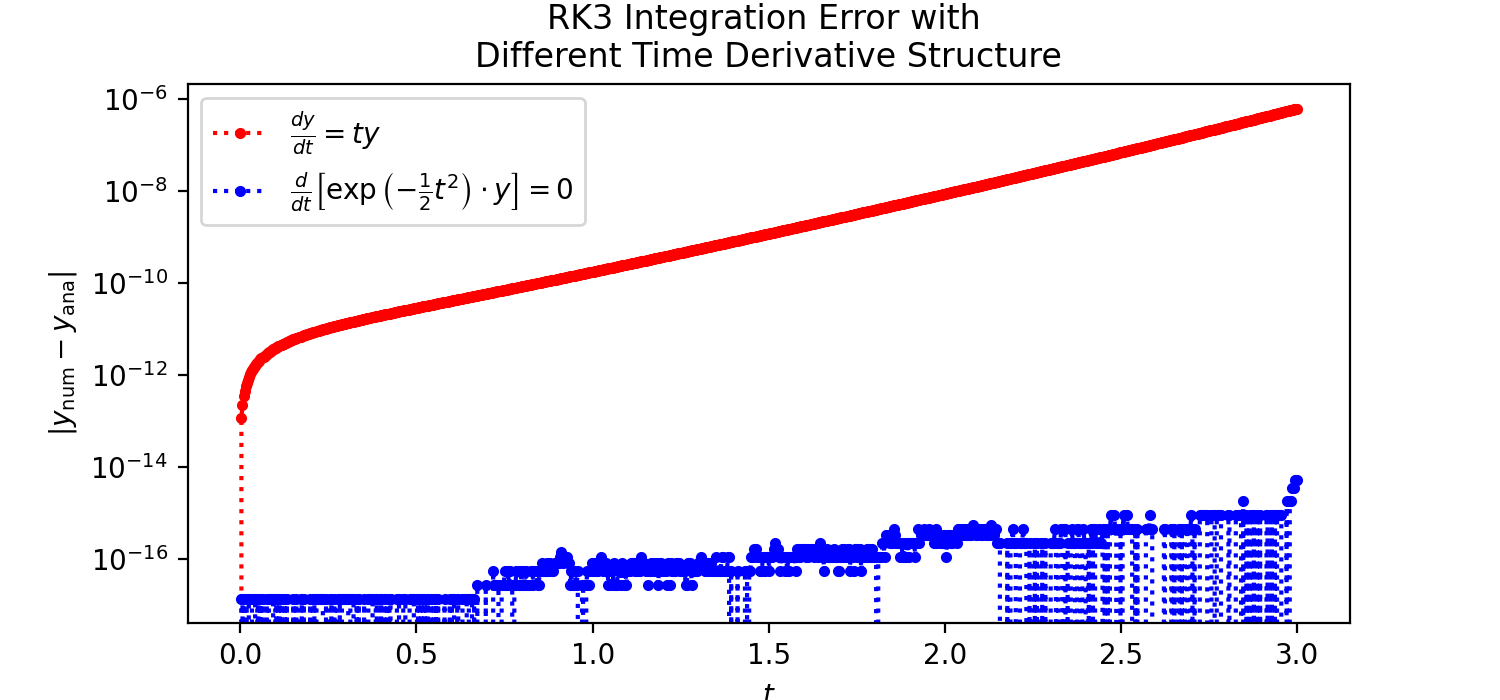
\includegraphics[width = 1\linewidth]{RK3 Error, Time Derivative Structure.png}
\end{figure}
This figure can be reproduced by executing the script \texttt{rk3\_error\_f\_structure.py} (runtime $<1$ s).

\subsection{Verification of Model Advection PDE}
The Advection Equation is a standard model PDE of advection-type problems, which is described by the following.
\begin{equation}
    \pdv{\theta}{t} + a \pdv{\theta}{x} = 0
\end{equation}
where $a$ is a constant fluid velocity, and $\theta$ represents some scalar transport variable, i.e.\ temperature, but note that this would represent no diffusivity. While it can be naturally extended to higher dimensions, we will first consider the 1D case, which has the analytical solution\footnote{Solving first-order linear PDEs such as this one can often be accomplished by utilizing the \href{https://en.wikipedia.org/wiki/Method_of_characteristics}{Method of Characteristics}.}:
\begin{equation}
    \theta(t, x) = \theta(0, x - at)
\end{equation}

We will show that with decreasing $\Delta t$, with a maximum prescribed by the CFL condition, that the error between the analytical and numerical solution goes to zero, with a variety of methods.

\begin{figure}[H]
    \centering
    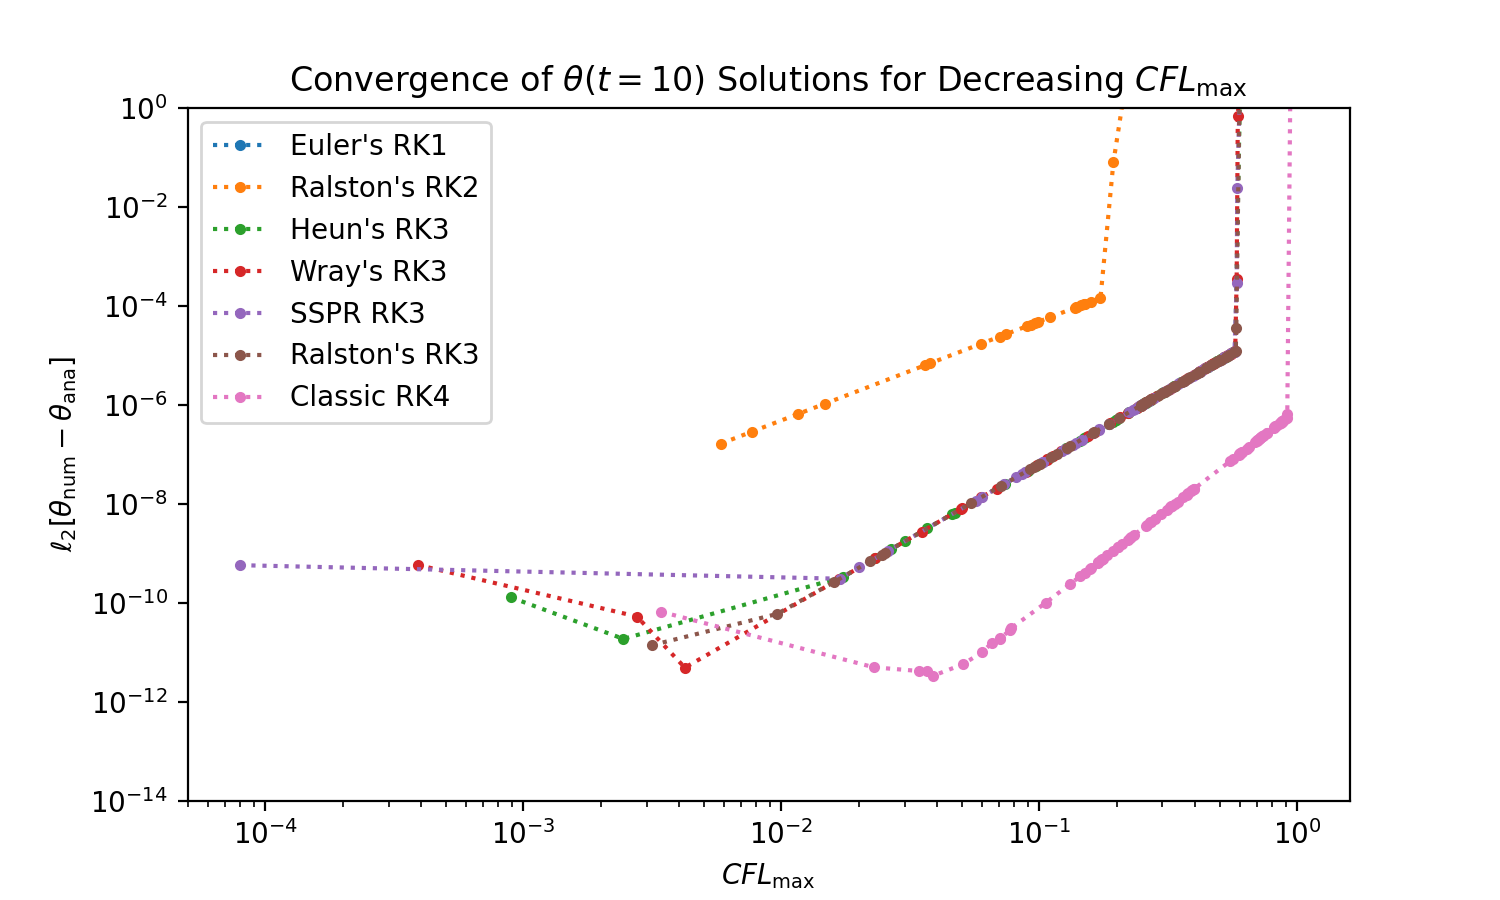
\includegraphics[width = 1\linewidth]{advection_error.png}
\end{figure}

It should be noted that Euler's RK1 and Ralston's RK2 are unstable for the advection equation, and integrating up to a higher time will show that for RK2 as well. The above figure can be replicated by executing \texttt{advection\_error.py} (runtime $<5$ m).

In order to determine the minimum RK scheme that will be stable, the eigenvalues of the differentiation matrix need to be found, and compared to the stability contours of RK schemes. For this advection problem (spectral or finite difference), the eigenvalues will be found solely on the imaginary axis in the complex plane. 

\begin{figure}[H]
    \centering
    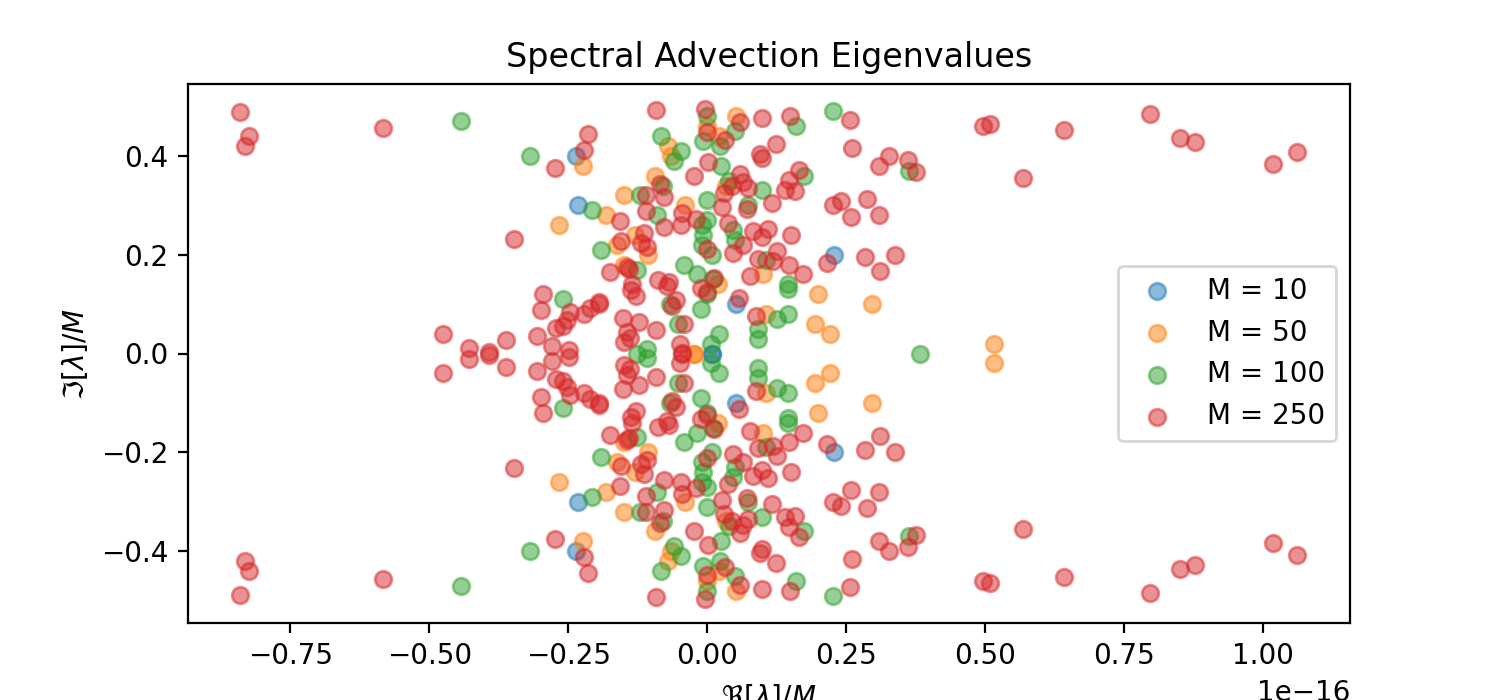
\includegraphics[width = 1\linewidth]{Spectral Eigenvalues.png}
\end{figure}

The derivation of the spectral differentiation matrix is not trivial. However, the above figure can be reproduced by executing \texttt{spectral\_eigenvalues.py} (runtime $<1$ s).

\subsection{Sandbox Test of Shock Evolution}
Though not directly relevent to the developement of the Voriticity-Streamfunction solver, shock evolution (and supersonic flow in general) were of particular interest to the developer. Burger's Equation, is a standard model PDE for shock-type problems.
\begin{equation}
    \pdv{u}{t} + u \pdv{u}{x} = \pdv{u}{t} + \frac{1}{2} \pdv{\left[u^2\right]}{x} = 0
\end{equation}
which are this equation's advective and conservative forms, respectively.

An explicit RK3 time-stepped, spectral-space solution of these two forms is almost identical, with the Advective form having very slightly less upwind oscillation. Regardless, both exhibit numerical instability and are not able evolve to a full shock. The following plot can be reproduced with \texttt{shock\_evolution.py} (runtime $< 5$ s).

\begin{figure}[H]
    \centering
    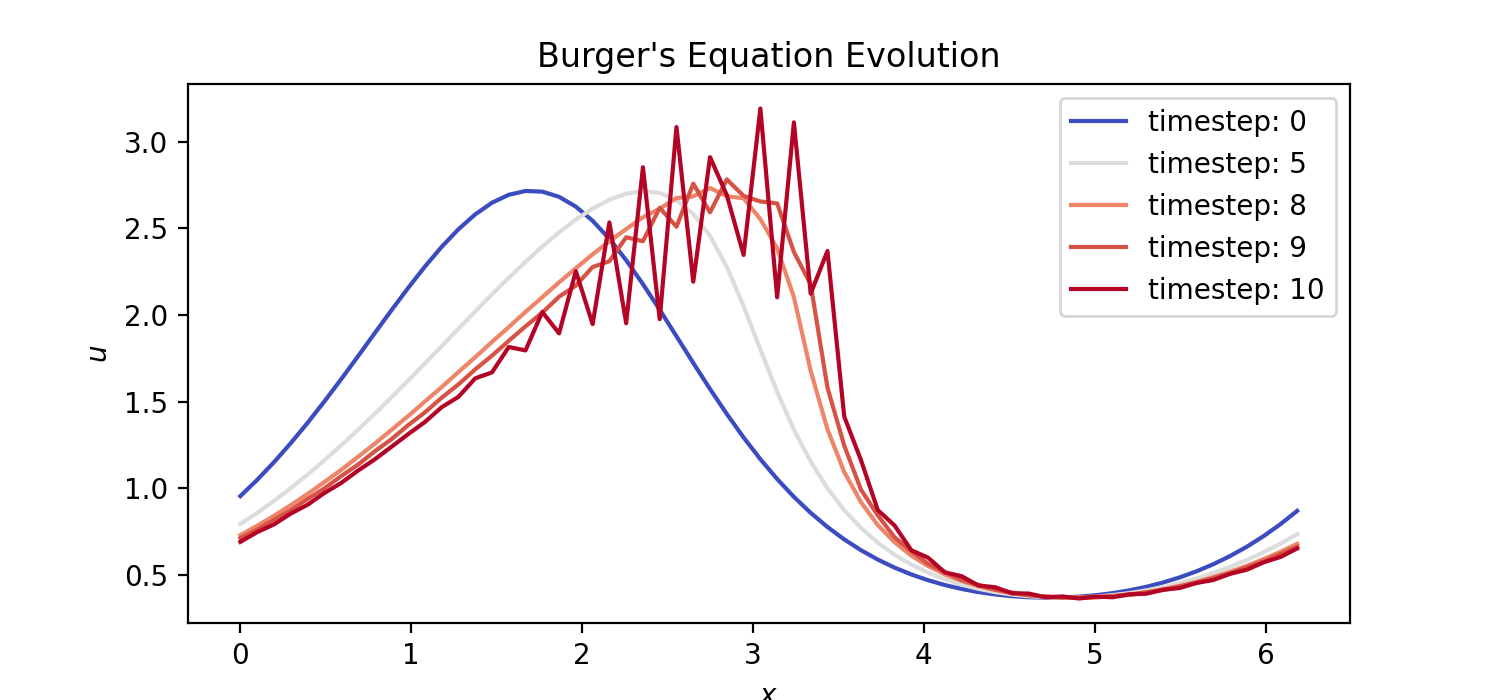
\includegraphics[width = 1\linewidth]{Burger's Equation Evolution.png}
\end{figure}

\subsection{Verification of Model Diffusion PDE}
The Heat Equation is a model PDE for diffusion-type problems, which the following form:
\begin{equation}
    \pdv{\theta}{t} = \nu \pdv[2]{\theta}{x}
\end{equation}
By assuming an initial condition with an analytical solution\footnote{The most common way to solve this type of PDE is to use \href{https://en.wikipedia.org/wiki/Separation_of_variables}{Seperation of Variables}.}, we can perform a convergence test to verify we can numerically solve this type of problem. Choosing an arbitrary initial condition:
\begin{equation}
    \theta(t = 0, x) = \sin(ax)
\end{equation}
\begin{equation}
    \theta(t, x) = e^{-\nu a^2 t} \sin(ax)
\end{equation}
The convergence test performs as expected. The following plot can be reproduced by running \texttt{heat\_error.py} (runtime $<5$ m).

\begin{figure}[H]
    \centering
    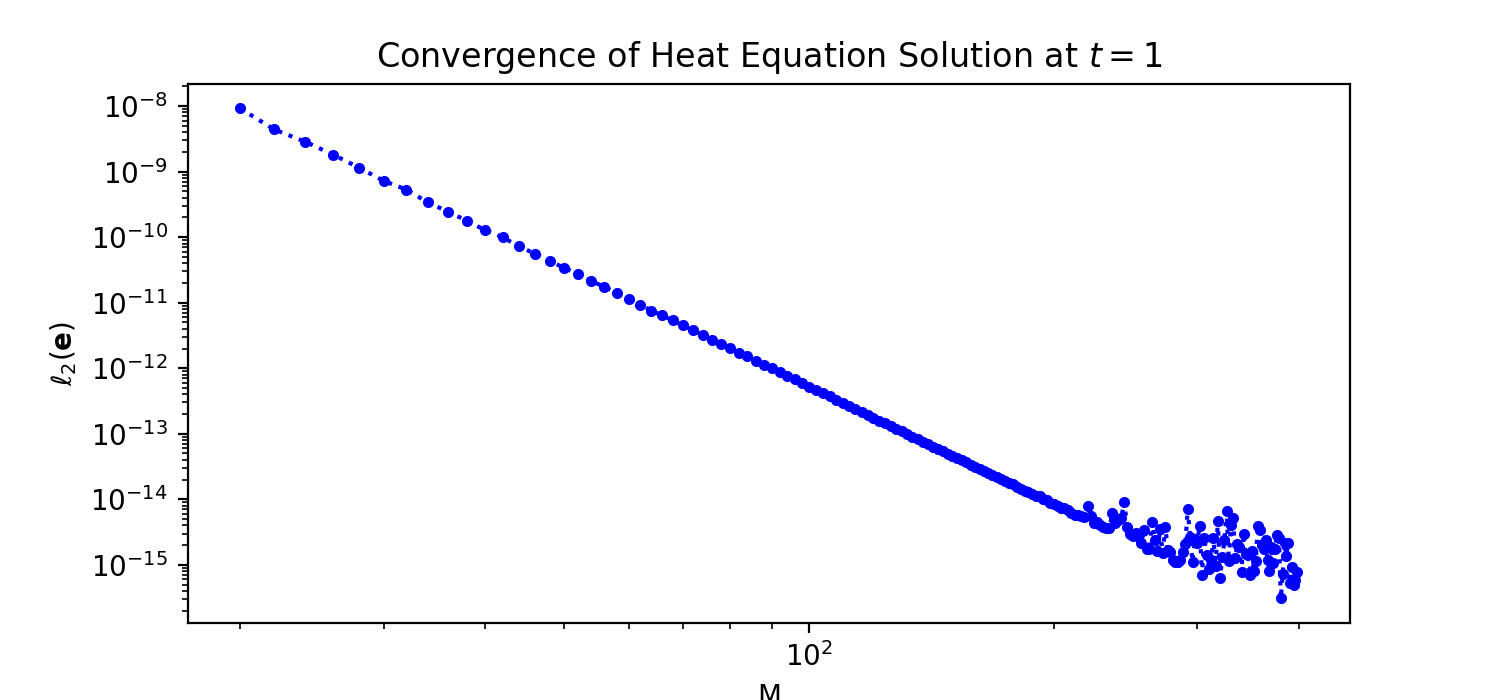
\includegraphics[width = 1\linewidth]{Heat Error.png}
\end{figure}

\subsection{Verification of Unperturbed Taylor-Green Flow}
As was stated previously, we initialize our Voriticity-Streamfunction solver as perturbed Taylor-Green flow. However, since Taylor-Green flow has an analytical solution, if we remove the perturbation, disable artificial viscosity forcing, and track the difference in solutions, we can verify if our solver is working correctly.

\begin{figure}[H]
    \centering
    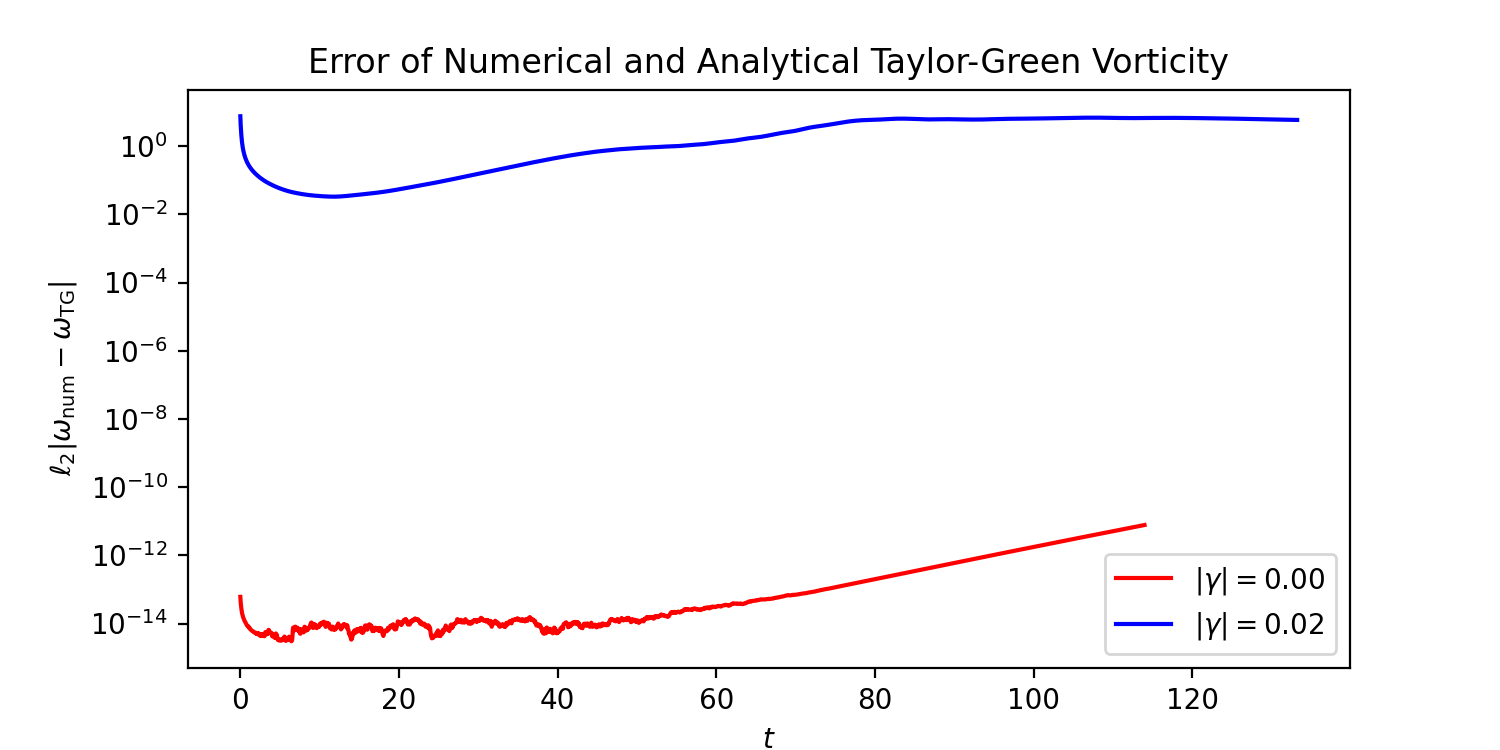
\includegraphics[width = 1\linewidth]{TG_verification_plot.png}
\end{figure}

It is interesting to note that even when there is no perturbation, numerical errors cause some level of `micro-turbulence' on the order of $10^{-12}$. This figure can be reproduced by running two instances of \texttt{TG\_verfication\_run.py} (runtime $<5$ m) with \texttt{gamma} set to $0.00$ and $0.02$, respectively. Afterwards, \texttt{TG\_verification\_plot.py} can be run (runtime $<25$ s).

\subsection{Verification of Non-Inertial Particle Transport}
In order to test our implementation of non-inertial particle transport, we will similarly use the Taylor-Green analytical solution. The positions for the streamlines, or lines with constant $\psi$ are unchanging in time, meaning, that a fluid particle will always follow a closed loop. As a result, if we transport a particle, and compare its streamfunction at the end of some integration period to its initial streamfunction value, we can determine the `drift' of the particle, or the Streamline Deviation.

\begin{figure}[H]
    \centering
    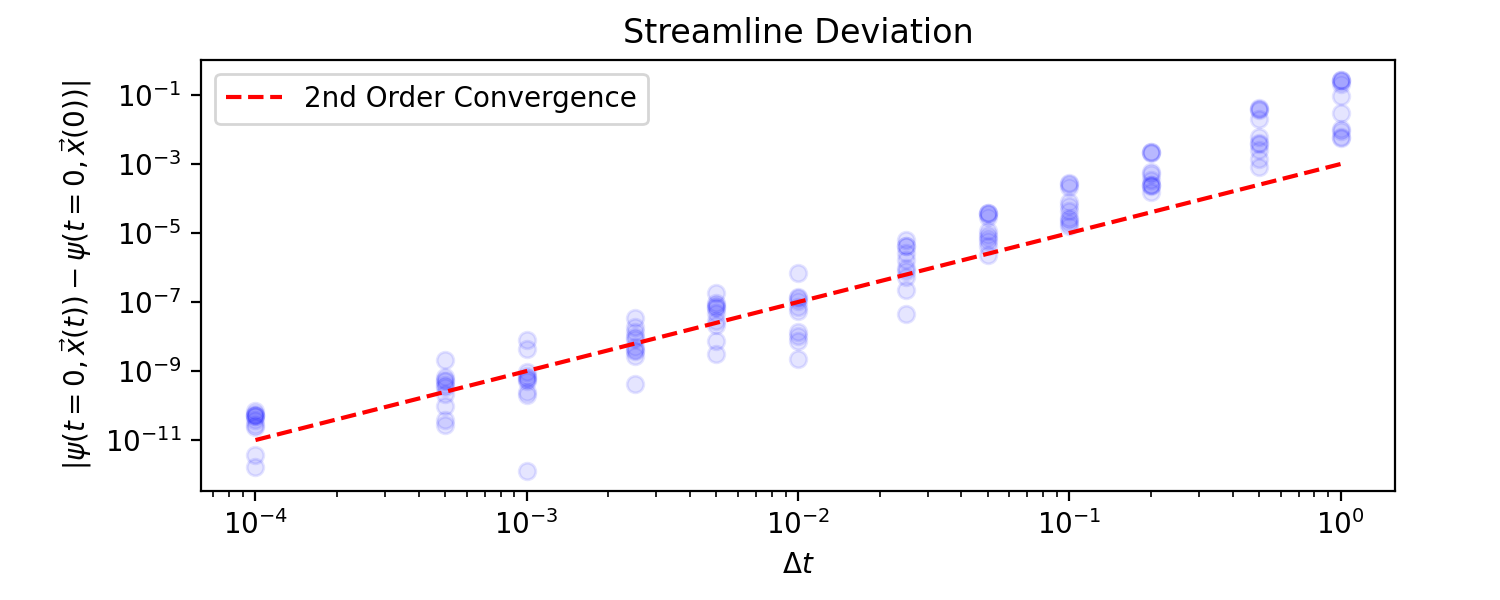
\includegraphics[width = 1\linewidth]{predictor-corrector_verification.png}
\end{figure}

It was shown that integrating up to time $t = 5$ and calculating the streamline deviation with decreasing $\Delta t$ yields 3rd-Order convergence. This figure can be reproduced by running \texttt{non-inertial\_verification.py} (runtime $< 10$ m).

\subsection{Verification of Inertial Particle Transport}
At the moment, no significant verification of inertial particle transport was completed.

\section{Continued Research}

\subsection{Passive Scalar Transport}
The transport equation for a passive, diffusing scalar variable, i.e. temperature, is as follows:
\begin{equation}
    \pdv{\theta}{t} + u_x \pdv{\theta}{x} + u_y \pdv{\theta}{y} + f(u_x, u_y) = \frac{\nu}{c} \left( \pdv[2]{\theta}{x} + \pdv[2]{\theta}{y} \right)
\end{equation}
where $f()$ is some arbitrary function that describes a constant scalar gradient, $c$ is a dimensionless variable that is the ratio of scalar diffusion to momentum diffusion (viscosity). For temperature, this is the Prandtl Number $\mathrm{Pr}$, for mass, this is the Schmidt Number $\mathrm{Sc}$, etc.

This was completed, though the code will not be shared (though one can perhaps dig through the entire folder if need be). With the skills developed by the reader in the process of reading and implementing what has been carefully described in this document, this scalar transport can be implemented relatively directly. 

Note: Plotting $\theta' = \theta - f(u_x, u_y)$ often results in a much better looking plot.

\begin{figure}[H]
    \centering
    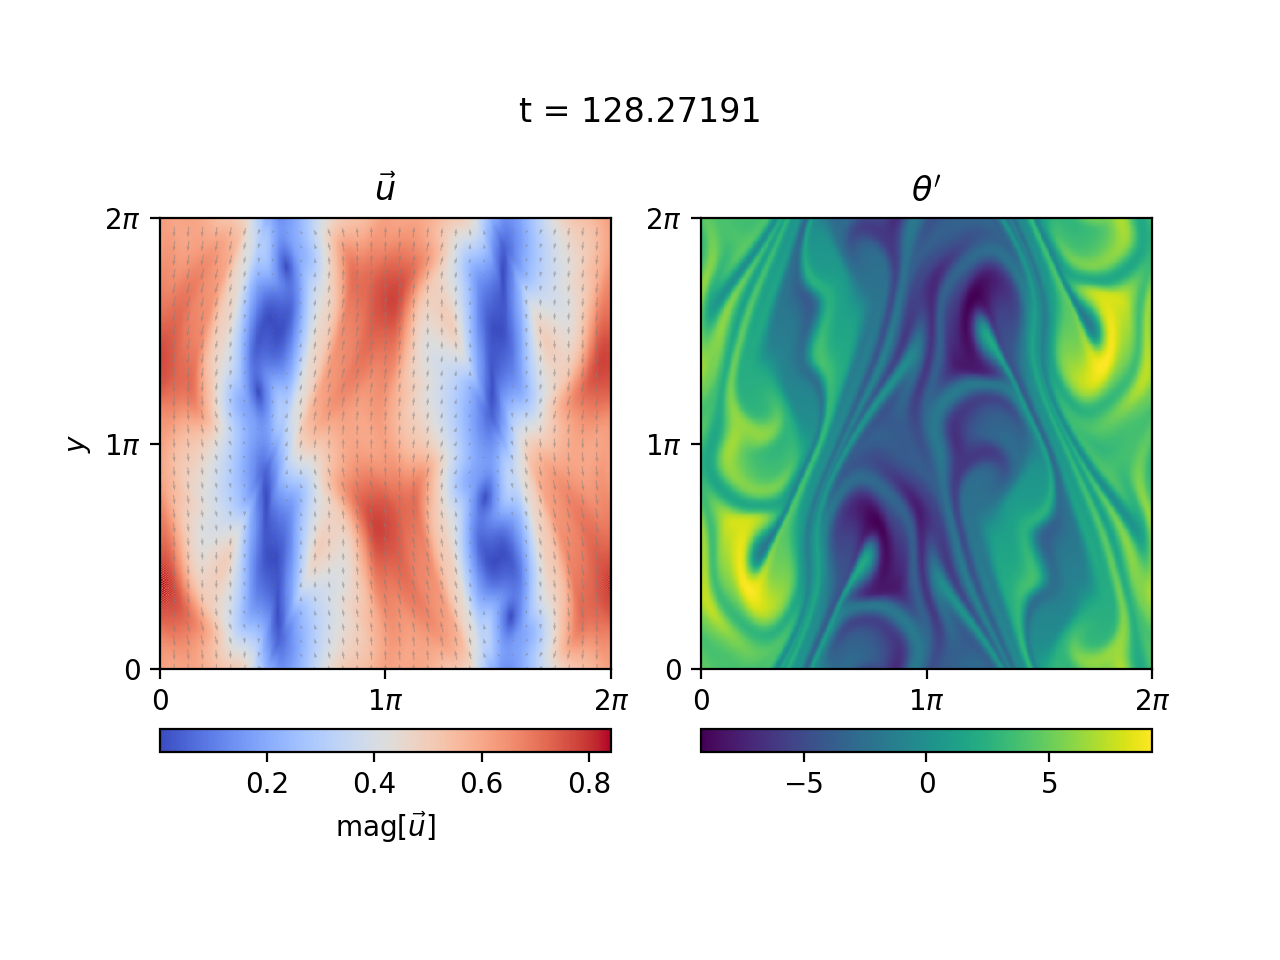
\includegraphics[width = 1\linewidth]{scalar_transport.png}
\end{figure}

\subsection{Binary Controlled Turbulent Kinetic Energy}
Without forcing, due to viscosity, the flow will naturally decay, even with perturbations. In order to sustain turbulence, an artificial viscosity can be implemented. 

Our viscous integrating factor $\Xi(t) = \exp [\nu(k_p^2 + k_q^2) t]$. We will define a slightly different version, where $\Xi_f(t) = \exp [\nu k_\Xi t]$. $k_\Xi$ is defined as:
\begin{equation}
    k_\Xi = \begin{cases}
        -k_p^2 - k_q^2, \quad 5^2 < k_p^2 + k_q^2 < 6^2 \\
        8(k_p^2 + k_q^2), \quad k_p^2 + k_q^2 < 4^2 \\
        +k_p^2 + k_q^2, \quad \mathrm{otherwise}
    \end{cases}
\end{equation}
This is non-physical, as it is equivalent to having viscosity be negative for very fine structures, and boosted for very large structures. This can be used, but numerical instability issues are difficult to control. As a result, a binary switch was implemented that uses the standard $k_p^2 + k_q^2$ when the turbulent kinetic energy $\mathrm{TKE}$ is greater than the initial condition, and $k_\Xi$ otherwise. The turbulent kinetic energy can be found as follows\footnote{The sum in physical and frequency space can be interchanged via \href{https://en.wikipedia.org/wiki/Parseval\%27s\_theorem}{Parceval's Thereom}}:
\begin{equation}
    \mathrm{TKE} = \sum_i \sum_j \left[ u_{x, ij}^2 + u_{y, ij}^2 \right] = \sum_p \sum_q \left[ |U_{x, pq}|^2 + |U_{y, pq}|^2 \right]
\end{equation}
However, even this seems plagued with odd instabilities. 

\begin{figure}[H]
    \centering
    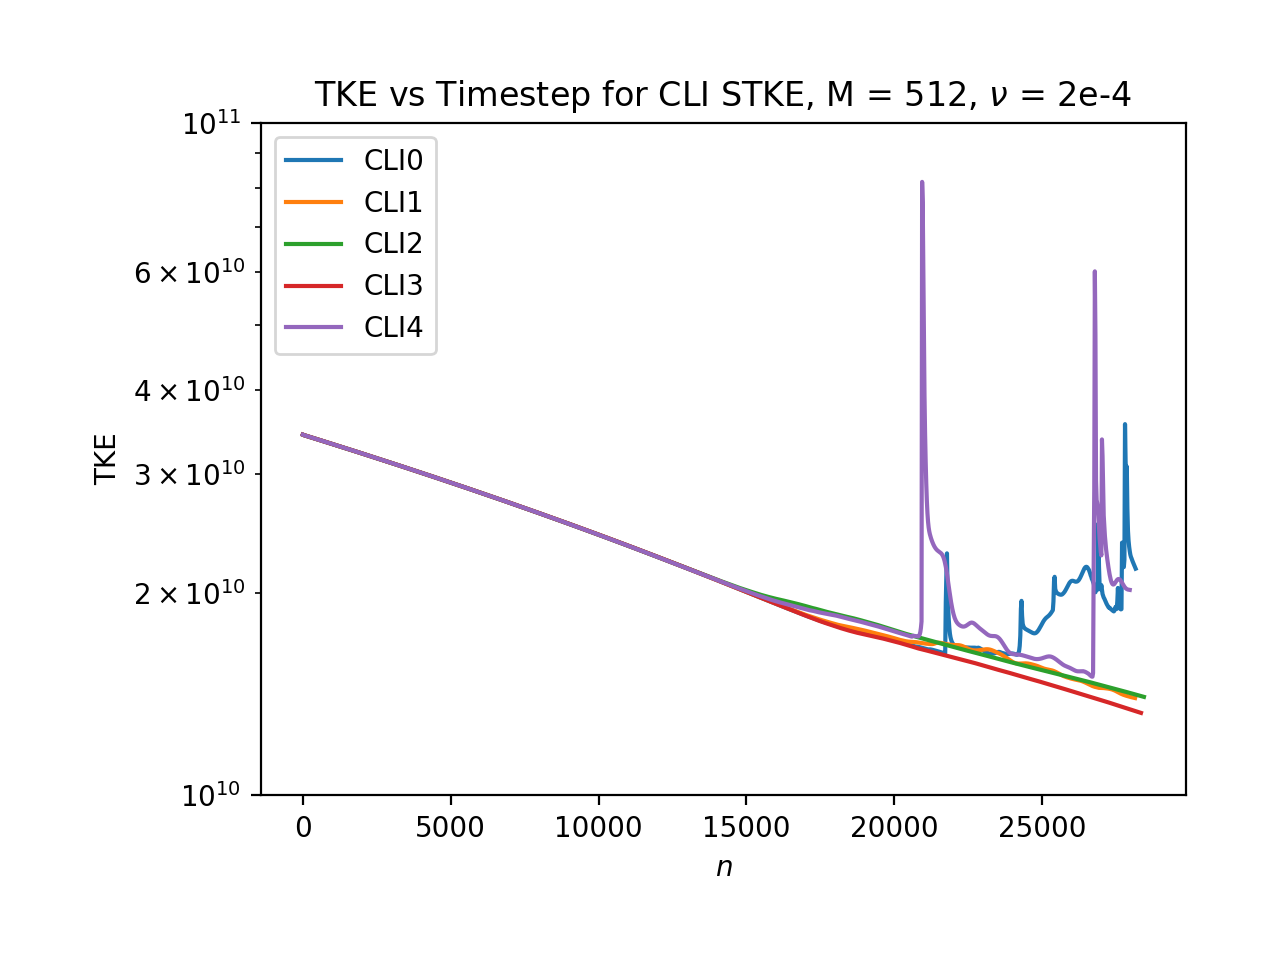
\includegraphics[width = 1\linewidth]{TKE Plot, 512.png}
\end{figure}
These instabilities were unfortunately not resolved, but they were well outside the scope of the initial goals of this project. Perhaps the reader may be able to resolve it.

\section{Conclusion}
Overall, this project was extremely helpful in helping me to develop skills in implementing a complex fluid dynamics method with almost no prior experience. I would like to thank Dr.\ Matheou for all his help during this project, as well as NIUVT for sponsoring this undergraduate research. I hope that this documentation serves to help the next researcher that will follow me.
\end{document}